\section{Experiment}
\label{sec:experiment}
In this section, we present experimental results for FlexMDM, demonstrating the following:
\begin{itemize}[leftmargin=*,itemsep=0pt,topsep=0pt]  
  \item \coloredhl{xxpurple}{FlexMDM is an effective variable-length learner}: length modeling, planning, local edits.
  \item \coloredhl{xsienna}{FlexMDM is scalable}: 8B FlexMDM is obtainable by initializing from a pretrained MDM.
\end{itemize}
Section~\ref{sec:experiment_pretrain} presents from-scratch results for FlexMDM on text and planning tasks distributions, confirming its practical efficiency. Next, Section~\ref{sec:experiment_llada} provides an 8B-scale FlexMDM's training recipe, initialized from LLaDA-8B \cite{nie2025large}, and evaluates it in math and code infilling tasks. We begin with the architectural and scheduling choices used throughout.

\begin{figure}[t]
    \vskip -3.0\baselineskip
    \centering
    \begin{subfigure}[t]{0.3\textwidth}
        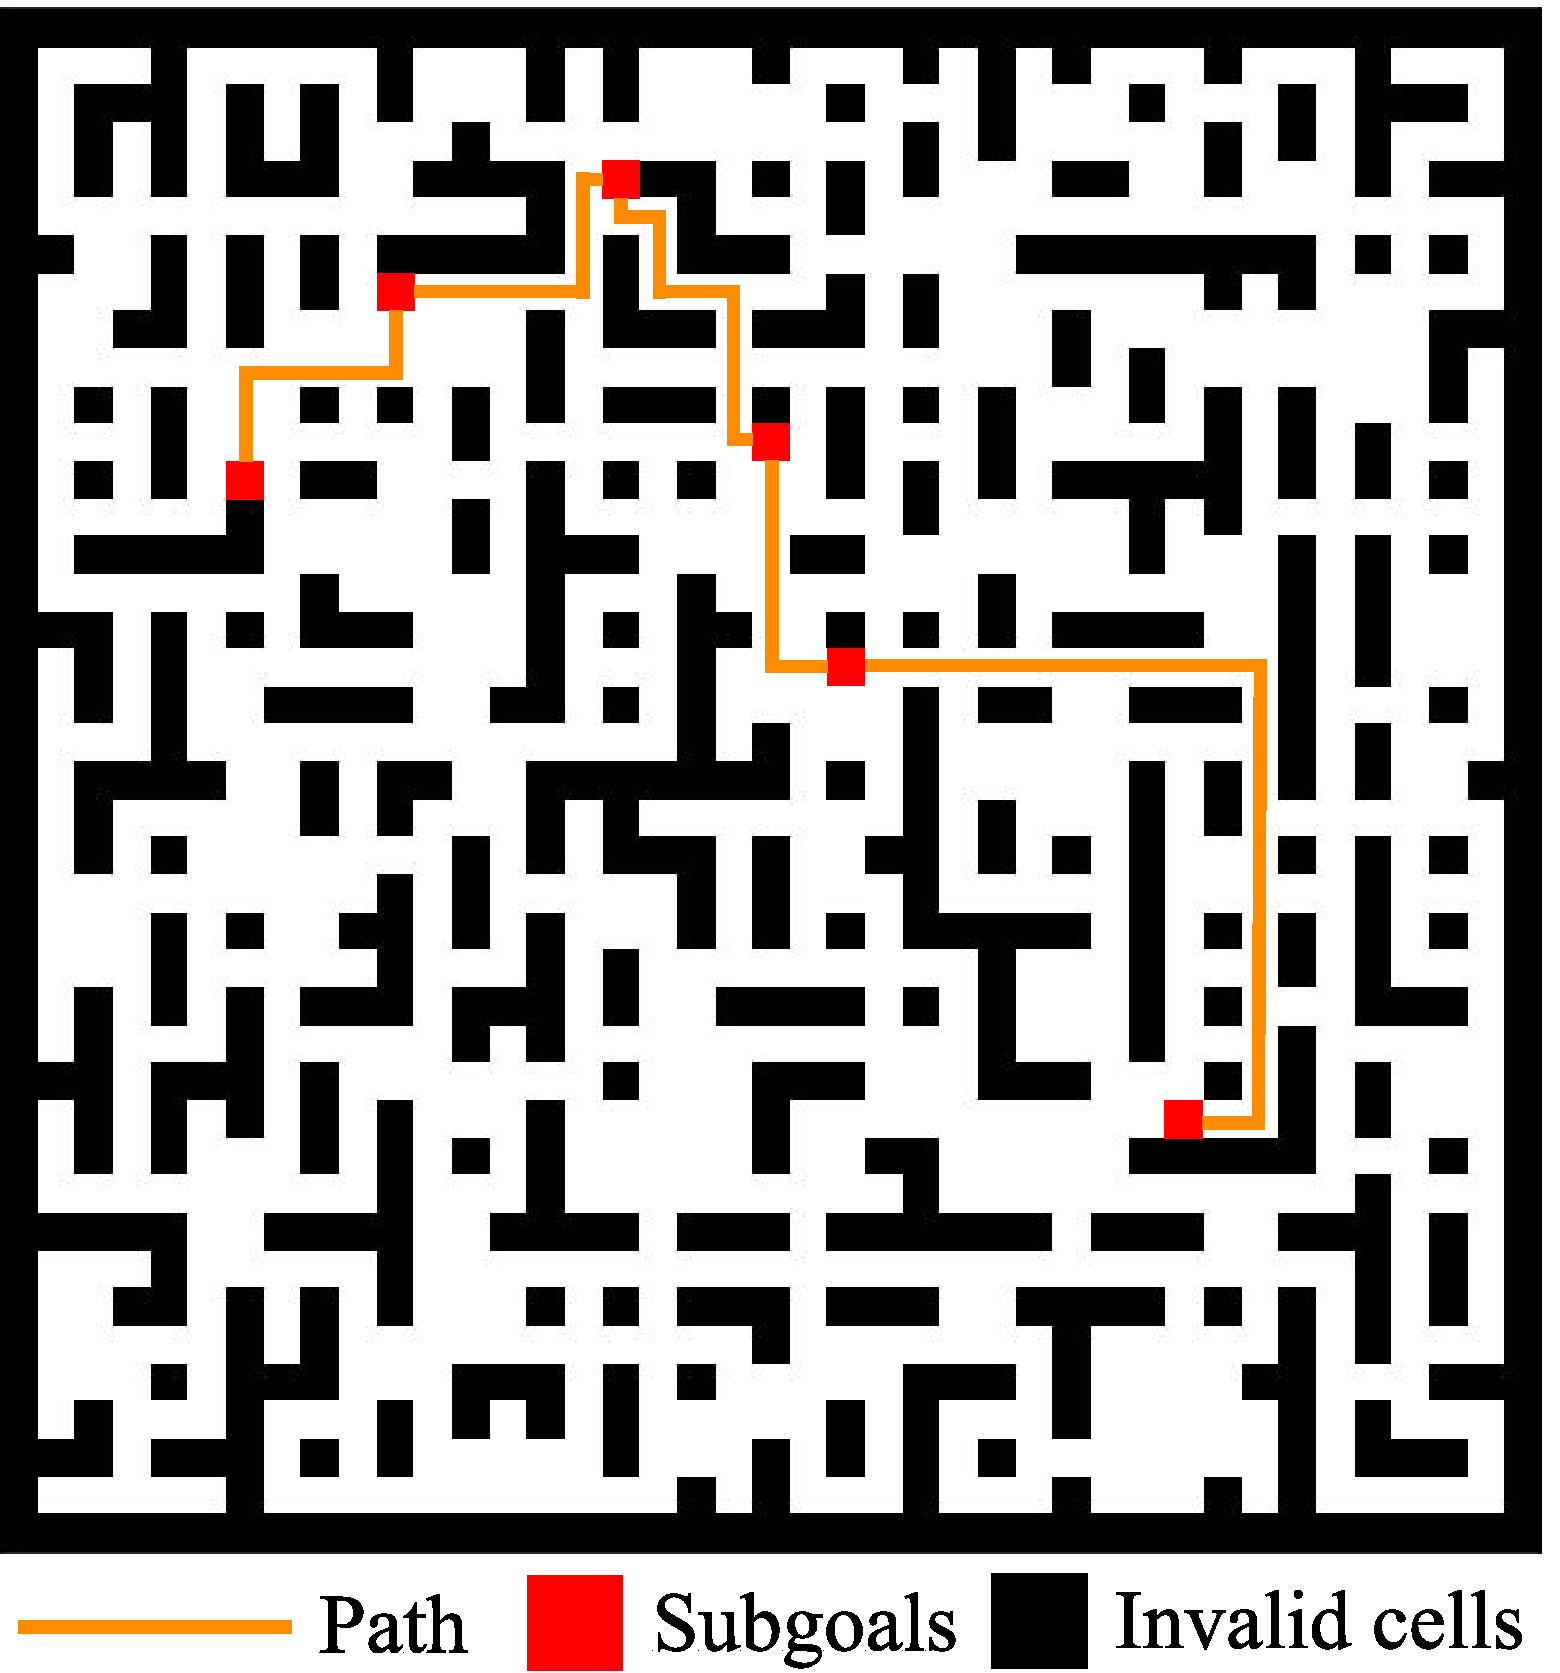
\includegraphics[height=0.99\textwidth]{Figures/maze_illus.pdf}
        \caption{\textbf{Maze task illustration.} The model is given subgoals and is required to connect them.} \label{fig:maze_illus}
    \end{subfigure}
    \hfill
    \begin{subfigure}[t]{0.33\textwidth}
        \centering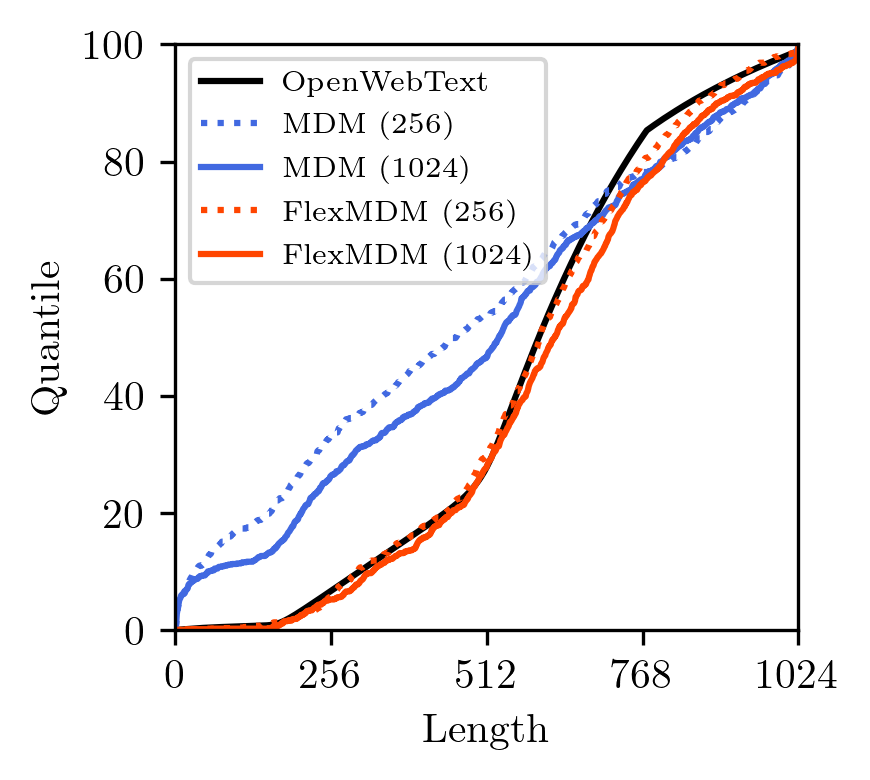
\includegraphics[scale=0.7,trim={0.6cm 0.4cm 0cm 0.0cm}]{Figures/length_quantiles.png}
        \caption{\textbf{Length modeling}. FlexMDM recovers the true length distribution of OpenWebText training data.} \label{fig:length_matching}
    \end{subfigure}
    \hfill
    \begin{subfigure}[t]{0.33\textwidth}
     \centering
        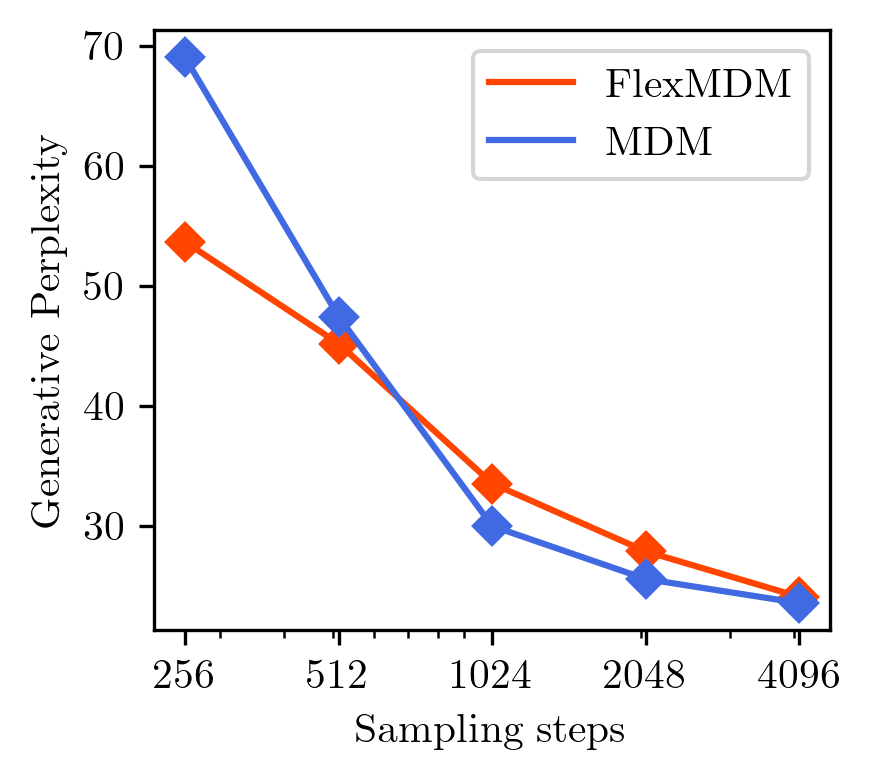
\includegraphics[scale=0.7,trim={0.6cm 0.4cm 0cm 0.0cm}]{Figures/gen_ppl_sampling_steps.png}
        \caption{\textbf{Perplexity.} FlexMDM achieves generative perplexity on par with MDM.} \label{fig:gen_ppl}
    \end{subfigure}
    \vskip -1.0\baselineskip
\end{figure}

\textbf{Training design.} Recall from Section~\ref{sec:FlexMDM_informal} that FlexMDM models the unmasking posterior $f_\theta$ and insertion expectation $g_\theta$ given state $x$ and time step $t$. We adopt DiT~\citep{peebles2023scalable}, a bidirectional transformer that enables additional embedding, as a backbone.
To learn both quantities jointly, we attach two output heads: a standard posterior head for $f_\theta$ and a scalar softplus head for $g_\theta$. Moreover, we choose our unmasking and insertion schedule to be both linear, $\alpha_t=\beta_t=t$\footnote{The ground-truth unmasking posterior is independent of $\beta_t$, so we condition the network on $\alpha_t$ only; under the linear choice $\alpha_t=t$, this coincides with the usual time embedding.}.

\subsection{Pretraining} \label{sec:experiment_pretrain}
In this section, we evaluate FlexMDM’s ability to learn variable-length data from scratch. Our baseline is MDM, which is fixed-length but can handle variable-length sequences by padding to a fixed maximum length with an auxiliary pad token. This padding setup is widely used in instruction fine-tuning when variable-length answers are desired~\citep{nie2025large,nie2024scaling,dream2025,gong2024scaling}. For a fair comparison, we use vanilla inference for both MDM and FlexMDM throughout. Further experimental details appear in Appendix~\ref{sec:appendix_exp_detail}.


\subsubsection{Pretraining on text data}
We first construct a training dataset from the raw OpenWebText corpus~\citep{Gokaslan2019OpenWeb}, splitting each article into paragraphs to preserve semantic coherence and yield variable-length sequences. Models pretrained on this data, therefore, generate variable-length text.

\textbf{Results.} We train $175$M FlexMDM and MDM with a maximum sequence length $1024$ for $500$K iterations and batch size $1024$. Using the pretrained models, we vary the number of sampling steps and measure (a) generative perplexity as a proxy for text fluency, and (b) the induced length distribution. Figure~\ref{fig:gen_ppl} shows comparative generative perplexity for the two models, improving as sampling steps increase, indicating no fluency degradation for FlexMDM despite its more involved loss objective. Crucially, we observe that \coloredul{xxpurple}{FlexMDM matches the true length distribution far more closely} (Figure~\ref{fig:length_matching}): with only $256$ steps it tracks the ground truth distribution (\coloreddashul{xred}{red line}, whereas MDM remains miscalibrated even at $1024$ steps (\coloredul{xblue}{blue line}).

\textbf{Remark.} We remark that our pretraining pipeline differs from prior MDM setups that truncate the corpus to a fixed maximum length. Also, one might ask why we do not provide additional metrics on text benchmarks, such as validation perplexity. This is because MDM and FlexMDM use different objectives (see equation~\eqref{eq:loss:mdm} and equation~\eqref{eq:FlexMDM_loss}), making likelihood comparisons hard to interpret. We address the concern about the absence of the metric by evaluating scaled models on downstream benchmarks in Section~\ref{sec:experiment_llada}.


\subsubsection{Planning task}
We further evaluate FlexMDM's ability in a planning task in a discrete space. Motivated by an earlier study \cite{janner2022diffuser} that investigated the ability of continuous diffusion in maze tasks, we design a grid-maze benchmark: the maze is fixed but unknown to the model, with a subset of cells invalid. Given a sequence of subgoal grids $(g_1,\dots,g_{K})$, the model must connect this sequence without entering invalid cells (see Figure~\ref{fig:maze_illus}). This subgoal structure aligns naturally with FlexMDM: starting from $(g_1,\dots,g_K)$, inference inserts mask tokens between subgoals and then unmasks to generate a feasible path. Theoretically, this can be seen as augmenting the base distribution to contain a data-dependent distribution \cite{albergo2024stochastic}. This is in stark contrast to MDM, where it must preassign each subgoal to a specific position, which is difficult to know \emph{a priori}. We provide additional details in Appendix~\ref{app:maze}.

\begin{minipage}{0.62\textwidth}
\textbf{Results.} We use a $41\times41$ maze and control the task's difficulty via varying the number of subgoals $K\in\{2,7,12\}$. As $K$ increases, MDM performance degrades markedly, while FlexMDM maintains robust success rates, \coloredul{xxpurple}{reaching a gap of up to $60\%$ at $K=12$}. These results firmly support FlexMDM as a principled approach for subgoal-based planning, where preallocating token positions is inherently challenging for fixed-length models.
\end{minipage}
\hfill
\begin{minipage}{0.35\textwidth}
\begin{table}[H]
    \centering
    \vspace{-0.08in}
    \begin{tabular}{lcc}
        \toprule
        \textbf{Difficulty} & \textbf{MDM} & \textbf{FlexMDM} \\
        \midrule
        Easy & 68.4\% & \textbf{92.3\%}  \\
        Medium & 29.3\% & \textbf{90.4\%}\\
        Hard & 24.2\% & \textbf{90.0\%} \\
        \bottomrule
    \end{tabular}
    \vspace{-0.1in}
     \caption{FlexMDM outperforms MDM on the subgoal-style maze-planning task.}
\end{table}
\end{minipage}

\subsection{Scaling up FlexMDM} \label{sec:experiment_llada}
In this section, we address FlexMDM's scalability by scaling it to 8B parameters and observing notable improvements over an MDM baseline. We start from the observation that MDM and FlexMDM both share the unmasking posterior as a core component, suggesting effective \emph{task transfer} from a pretrained MDM might be possible. To demonstrate this, concretely, we initialize from LLaDA-Base~\citep{nie2025large} and make the following modifications: (a) add time-embedding layers and a scalar head to model the insertion expectation; (b) attach LoRA adapters. Altogether, the resulting number of trainable parameters is $\approx$400M. To cover both natural and mathematical language, we train on the 50:50 mixture of OpenWebText~\citep{Gokaslan2019OpenWeb} and Proof-Pile-2~\citep{azerbayev2023llemma}. Surprisingly, \coloredul{xsienna}{we observe rapid transfer}: within three days on $16$ H100 GPUs, the model generates variable-length sentences. We then instruction-fine-tune (IFT) this base FlexMDM to evaluate it on downstream tasks. See Appendix \ref{sec:appendix_exp_detail} for more details \footnote{For a fair comparison, since FlexMDM is not IFT-ed, we IFT LLaDA-Base, rather LLaDA-instruct, this differs from \cite{zhao2025d1}. We employ zero-shot evaluation, which also differs from \cite{nie2024scaling}.} 

\textbf{Results.} For comparison, we train FlexMDM and LLaDA-Base from the same number of IFT pairs. For math and code, respectively, we IFT on the GSM8K train split(\cite{cobbe2021training}; $\approx$8000 pairs) and the educational split of opc-sft-stage-2~\citep{Huang2024OpenCoderTO} ($\approx$0.1M pairs), for which IFT-ed models are evaluated in the GSM8K test split and HumanEval-infill (single line)~\citep{bavarian2022efficient} in zero-shot. Sampling is done by confidence-based sampling with a sliding window. Notably, as the number of sampling steps increases, \coloredul{xsienna}{FlexMDM continues to improve}, highlighting its strength in \coloredul{xsienna}{reasoning tasks} given sufficient compute—whereas the IFT-ed LLaDA’s performance remains flat. Although in this experiment we use IFT on task-specific pairs, we expect that training on a much more diverse instruction–answer pairs with sufficient compute will yield a more generalized model.
%
\hfill
\begin{figure}[H]
    \centering
    \vskip -1.0\baselineskip
    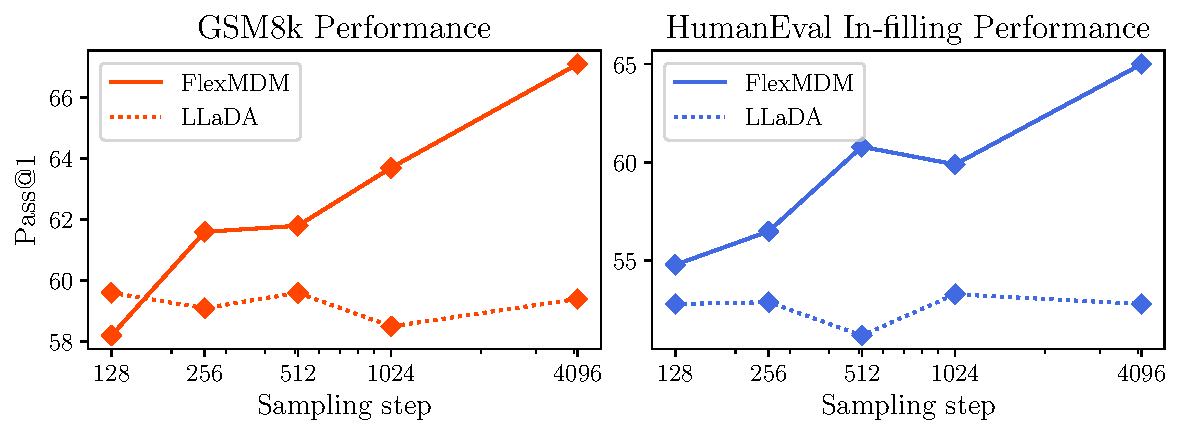
\includegraphics[width=0.9\textwidth,trim={0.5cm 0 0.2cm 0}]{Figures/math_code.pdf}
    \vskip -1.0\baselineskip
    \caption{FlexMDM performance exhibits superior scaling when more sampling steps are allocated.}
\end{figure}
\vspace{-0.2in}